%!TEX root = ../Dokumentation.tex
\chapter{Projektreflektion}
In der zweiten Projektphase des Sommersemesters 2013 im Modul Web-basierte Anwendungen 2, ging es um die Realisierung eines verteilten Systems. Zu Beginn dieser Dokumentation wurde das Konzept des SerienTrackers vorgestellt. Das wurden verschiedene Möglichkeiten zum Informationsaustausch angedacht und die verschiedenen Kommunikationsmöglichkeiten überlegt. Es folgte eine Vorstellung der einzelnen Entwicklungsphasen mit Ergebnissen, Ideen und einigen Alternativansätzen.\\


Wie bereits an manchen Stellen während der Ausarbeitung angesprochen, verlief die Entwicklung teilweise etwas anders als geplant. Zu Beginn stand bereits die Frage offen, ob die Einbindung eines Freundefeatures zeitlich realisierbar ist. Spätens im 3. Meilenstein des RESTful Webservice, wurde dieser Aspekt bereits zurückgestellt und auch andere Features woe Bewertungen oder Fehlermeldungen sind nach Ablauf der Projektphase nicht umgesetzt.
Zugunsten zahlreicher Features viel die Konzentration deshalb auf einige wenige und diese wurden zur Vertiefung in den Fokus gerückt.
Im Laufe des Projektes machte sich der recht knappe Zeitplan deutlich bemerkbar,speziell bei den späteren Meilensteinen, bei welchen vor der Ausarbeitung der Grundlagenstoff vertieft werden muss. Eine kontinuerliche Beschäftigung mit den jeweiligen Inhalten ist in diesem Fall notwendig und vereinfacht einen Teil der Organisation. Ein simples Aufschieben von Aufgaben war auch aufgrund der Präsenztermine nicht möglich, was jedoch zum Fortschritt beitrug. Diese Herangehensweise war prinzipiell schon aus vorherigen Projekten bekannt, in diesem Fall aber unvermeindlich und soll auch in späteren Projekten angestrebt werden.
Die grafische Darstellung zur Codefrequenz auf GitHub, zeigt noch, dass innerhalb des Projektes speziell in der mittleren Phase deutlich mehr Potential steckte. 

\begin{figure}[H]
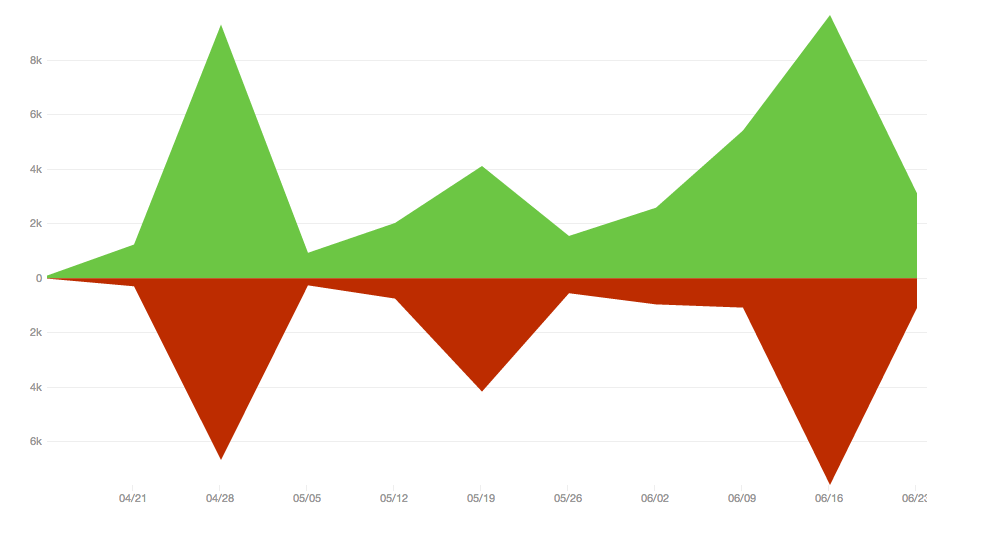
\includegraphics[width=1\textwidth]{../images/statistik}
\caption{Codefrequency GitHub }
\label{codefrequency}
\end{figure}

Auch die Verwendung von GitHub als Versionskontrolle stellte zur Projektentwicklung eine gute Unterstützung dar. Austausch von Codes und anderen Dateien fand auf diesem Weg in einer sehr effektiven Form statt und soll für zukünftige Projekte erneut verwendet werden. Regelmäßige Absprachen und gemeinsames Arbeiten, förderte dabei den Lernfortschritt.\\
Was das finale Ergebnis angeht, so wurde keinesfalls das zuvor angestrebte Ergebnis erfüllt. Dieses war jedoch deutlich zu hoch angesetzt, was den Umfang anging und zwischendurch auftretende Probleme wirkten sich im Zeitrahmen als Hindernis auf.
Dennoch wurde sich den Anforderungen entsprechend mit den jeweiligen Projektzielen beschäftigt, sodass das die Lernziele umgesetzt und verstanden werden konnten.\\

In Anbetracht auf zukünftige Projekte, speziell das Entwicklungsprojekt interaktive Systeme im nächsten Semester, brachte dieses Projekte lehrreiches Wissen und zeigte Stellen auf, an denen noch mehr Potential steckt. 

\newpage
